\newcommand{\titulus}{\nomenFesti{Dominica VI quæ superfuit post Epiphaniam.}
\celebratio{Semiduplex.}} \newcommand{\tedeumromanum}{Romanum}
\newcommand{\magnificati}{\pars{Canticum B. Mariæ V.} \scriptura{Dan. 3, 54.55.56; \textbf{H420}}

\vspace{-7mm}

{
\grechangedim{interwordspacetext}{0.18 cm plus 0.15 cm minus 0.05 cm}{scalable}%
\antiphona{I D\textsuperscript{2}}{temporalia/ant-quicaelorumcontines.gtex}
\grechangedim{interwordspacetext}{0.22 cm plus 0.15 cm minus 0.05 cm}{scalable}%
}

%\trAntIMagnificat

\vspace{-3mm}

\scriptura{Lc. 1, 46-55}

\vspace{-2mm}

\cantusSineNeumas
\initiumpsalmi{temporalia/magnificat-initium-isoll-D2.gtex}

\vspace{-1.5mm}

\input{temporalia/magnificat-isoll-D2.tex} \Abardot{}}
\newcommand{\lectioi}{\pars{Lectio I.} \scriptura{Os. 1, 1-3}

\noindent Incipit liber Osée Prophétæ.

\noindent Verbum Dómini, quod factum est ad Osée, fílium Béeri, in diébus Ozíæ, Ióathan, Achaz, Ezechíæ, regum Iuda; et in diébus Ieróboam, fílii Ioas, regis Israël. Princípium loquéndi Dómino in Osée. Et dixit Dóminus ad Osée: Vade, sume tibi uxórem fornicatiónum, quia fórnicans fornicábitur terra a Dómino. Et ábiit, et accépit Gomer, fíliam Debélaim: et concépit, et péperit ei fílium.}
\newcommand{\responsoriumi}{\pars{Responsorium 1.} \scriptura{\Rbardot{} Is. 6, 1 \Vbardot{} Is. 6, 2; \textbf{H416}}

\vspace{-5mm}

\responsorium{I}{temporalia/resp-vididominumsedentem-CROCHU-sinedox.gtex}{}}
\newcommand{\lectioii}{\pars{Lectio II.} \scriptura{Os. 1, 4-7}

\noindent Et dixit Dóminus ad eum: Voca nomen eius Iézrahel, quóniam adhuc módicum, et visitábo sánguinem Iézrahel super domum Iehu, et quiéscere fáciam regnum domus Israël, et in illa die cónteram arcum Israël in valle Iézrahel. Et concépit adhuc, et péperit fíliam. Et dixit ei: Voca nomen eius Absque misericórdia, quia non addam ultra miseréri dómui Israël, sed oblivióne oblivíscar eórum, et dómui Iuda miserébor et salvábo eos in Dómino Deo suo; et non salvábo eos in arcu et gládio, et in bello, et in equis, et in equítibus.}
\newcommand{\responsoriumii}{\pars{Responsorium 2.} \scriptura{\Rbardot{} Dan. 9, 18 \Vbardot{} Ps. 79, 2; \textbf{H416}}

\vspace{-5mm}

\responsorium{I}{temporalia/resp-aspicedominedesede-CROCHU.gtex}{}}
\newcommand{\lectioiii}{\pars{Lectio III.} \scriptura{Os. 1, 8-11}

\noindent Et ablactávit eam quæ erat Absque misericórdia, et concépit, et péperit fílium. Et dixit: Voca nomen eius, Non pópulus meus, quia vos non pópulus meus, et ego non ero vester. Et erit númerus filiórum Israël quasi aréna maris, quæ sine mensúra est, et non numerábitur. Et erit, in loco ubi dicétur eis: Non pópulus meus vos; dicétur eis: Fílii Dei vivéntis. Et congregabúntur fílii Iuda et fílii Israël páriter: et ponent síbimet caput unum, et ascéndent de terra, quia magnus dies Iézrahel.}
\newcommand{\responsoriumiii}{\pars{Responsorium 3.} \scriptura{\Rbardot{} Dan. 3, 55; Is. 40, 12 \Vbardot{} Ps. 79, 2; Dan. 9, 18; \textbf{H419}}

\vspace{-5mm}

\responsorium{II}{temporalia/resp-quicaelorumcontinesthronos-CROCHU-cumdox.gtex}{}}
\newcommand{\lectioiv}{\pars{Lectio IV.} \scriptura{Liber 18, cap. 28.}

\noindent Ex libro sancti Augustíni Epíscopi de Civitáte Dei.

\noindent Osée prophéta, quanto profúndius quidem lóquitur, tanto operósius penetrátur. Sed áliquid inde suméndum est, et hic ex nostra promissióne ponéndum. Et erit, inquit, in loco quo dictum est eis, Non pópulus meus vos; vocabúntur et ipsi fílii Dei vivi. Hoc testimónium prophéticum de vocatióne pópuli Géntium, qui prius non pertinébat ad Deum, étiam Apóstoli intellexérunt.}
\newcommand{\responsoriumiv}{\pars{Responsorium 4.} \scriptura{\Rbardot{} Is. 62, 6 \Vbardot{} ibid. 66, 19; \textbf{H417}}

\vspace{-5mm}

\responsorium{VI}{temporalia/resp-supermurostuos-CROCHU.gtex}{}}
\newcommand{\lectiov}{\pars{Lectio V.}

\noindent Et quia ipse quoque pópulus Géntium spiritáliter est in fíliis Abrahæ, ac per hoc recte dícitur Israël; proptérea séquitur, et dicit: Et congregabúntur fílii Iuda et fílii Israël in idípsum, et ponent síbimet principátum unum, et ascéndent a terra. Hoc si adhuc velímus expónere, elóquii prophétici obtundétur sapor. Recolátur tamen lapis ille anguláris, et duo illi paríetes, unus ex Iudǽis, alter ex Géntibus: ille nómine filiórum Iuda, iste nómine filiórum Israël, eídem uni principátui suo in idípsum inniténtes, et ascendéntes agnoscántur in terra.}
\newcommand{\responsoriumv}{\pars{Responsorium 5.} \scriptura{\Rbardot{} Ps. 54, 10 \Vbardot{} Ier. 14, 19; \textbf{H419}}

\vspace{-5mm}

\responsorium{III}{temporalia/resp-praecipitadomine-CROCHU.gtex}{}}
\newcommand{\lectiovi}{\pars{Lectio VI.}

\noindent Istos autem carnáles Israëlítas, qui nunc nolunt crédere in Christum, póstea creditúros, id est fílios eórum, (nam útique isti in suum locum moriéndo transíbunt) idem prophéta testátur, dicens: Quóniam diébus multis sedébunt fílii Israël sine rege, sine príncipe, sine sacrifício, sine altári, sine sacerdótio, sine manifestatiónibus. Quis non vídeat, nunc sic esse Iudǽos?}
\newcommand{\responsoriumvi}{\pars{Responsorium 6.} \scriptura{\Rbardot{} Ier. 14, 19.20 \Vbardot{} Bar. 2, 12; \textbf{H417}}

\vspace{-5mm}

\responsorium{VIII}{temporalia/resp-sustinuimuspacemetnonvenit-CROCHU-cumdox.gtex}{}}
\newcommand{\lectiovii}{\pars{Lectio VII.} \scriptura{Mt. 13, 31-35}

\noindent Léctio sancti Evangélii secúndum Matthǽum.

\noindent In illo témpore: Dixit Iesus turbis parábolam hanc: Símile est regnum cælórum grano sinápis, quod accípiens homo seminávit in agro suo.  Et réliqua.

\scriptura{Lib. 2. Comment. in cap. 13. Matth.}

\noindent Homilía sancti Hierónymi Presbýteri.

\noindent Regnum cælórum prædicátio Evangélii est, et notítia Scripturárum, quæ ducit ad vitam, et de qua dícitur ad Iudǽos: Auferétur a vobis regnum Dei, et dábitur genti faciénti fructus eius. Símile est ergo huiuscémodi regnum grano sinápis, quod accípiens homo seminávit in agro suo. Homo qui séminat in agro suo, a plerísque Salvátor intellégitur, quod in ánimis credéntium séminet: ab áliis ipse homo séminans in agro suo, hoc est in semetípso, et in corde suo.}
\newcommand{\responsoriumvii}{\pars{Responsorium 7.} \scriptura{\Rbardot{} Is. 19, 25 \Vbardot{} Ps. 32, 12; \textbf{H418}}

\vspace{-5mm}

\responsorium{VIII}{temporalia/resp-laudabilispopulus-CROCHU.gtex}{}}
\newcommand{\lectioviii}{\pars{Lectio VIII.}

\noindent Quis est iste, qui séminat, nisi sensus noster et ánimus; qui suscípiens granum prædicatiónis, et fovens seméntem, humóre fídei facit in agro sui péctoris pulluláre? Prædicátio Evangélii mínima est ómnibus disciplínis. Ad primam quippe doctrínam, fidem non habet veritátis, hóminem Deum, Christum mórtuum, et scándalum crucis prǽdicans. Confer huiuscémodi doctrínam dogmátibus philosophórum, et libris eórum, et splendóri eloquéntiæ, et compositióni sermónum: et vidébis quanto minor sit céteris semínibus seméntis Evangélii.}
\newcommand{\responsoriumviii}{\pars{Responsorium 8.} \scriptura{\Rbardot{} Is. 6, 3 \Vbardot{} Io. 5, 7; \textbf{Bud.\textsuperscript{118} 111v.}}

\vspace{-5mm}

\responsorium{I}{temporalia/resp-duoseraphim-cumdox.gtex}{}}
\newcommand{\lectioix}{\pars{Lectio IX.}

\noindent Sed illa cum créverint, nihil mordax, nihil vívidum, nihil vitále demónstrant: sed totum fláccidum marcidúmque et mollítum ebúllit in ólera et in herbas, quæ cito aréscunt et córruunt. Hæc autem prædicátio, quæ parva videbátur in princípio, cum vel in ánima credéntis, vel in tot mundo sata fúerit, non exsúrgit in ólera, sed crescit in árborem: ita ut vólucres cæli (quas vel ánimas credéntium, vel fortitúdines, Dei servítio mancipátas, sentíre debémus) véniant et hábitent in ramis eius. Ramos puto evangélicæ árboris, quæ de grano sinápis créverit, dógmatum esse diversitátes, in quibus supradictárum vólucrum unaquǽque requiéscit.}
\newcommand{\benedictus}{\pars{Canticum Zachariæ.} \scriptura{Mt. 25, 20; \textbf{H380}}

\vspace{-4mm}

{
\grechangedim{interwordspacetext}{0.18 cm plus 0.15 cm minus 0.05 cm}{scalable}%
\antiphona{I g}{temporalia/ant-dominequinquetalenta.gtex}
\grechangedim{interwordspacetext}{0.22 cm plus 0.15 cm minus 0.05 cm}{scalable}%
}

%\trAntIMagnificat

\vspace{-1mm}

\scriptura{Lc. 1, 68-79}

\vspace{-1mm}

\cantusSineNeumas
\initiumpsalmi{temporalia/benedictus-initium-isoll-g-auto.gtex}

%\vspace{-1.5mm}

\input{temporalia/benedictus-isoll-g.tex} \Abardot{}}
\newcommand{\magnificatii}{\pars{Canticum B. Mariæ V.} \scriptura{Mt. 25, 21; \textbf{H381}}

\vspace{-6mm}

{
\grechangedim{interwordspacetext}{0.18 cm plus 0.15 cm minus 0.05 cm}{scalable}%
\antiphona{IV E}{temporalia/ant-serveboneetfidelisquia.gtex}
\grechangedim{interwordspacetext}{0.22 cm plus 0.15 cm minus 0.05 cm}{scalable}%
}

%\trAntIMagnificat

\vspace{-1mm}

\scriptura{Lc. 1, 46-55}

\vspace{-2mm}

\cantusSineNeumas
\initiumpsalmi{temporalia/magnificat-initium-ivsoll-E.gtex}

%\vspace{-1.5mm}

\input{temporalia/magnificat-ivsoll-E.tex} \Abardot{}}
\newcommand{\hebdomada}{infra Hebdom. VI quæ superfuit post Epiphaniam.}
\newcommand{\oratioLaudes}{\cuminitiali{}{temporalia/oratio6pe.gtex}}
\newcommand{\hiemalis}{Hiemalis.}

% LuaLaTeX

\documentclass[a4paper, twoside, 12pt]{article}
\usepackage[latin]{babel}
%\usepackage[landscape, left=3cm, right=1.5cm, top=2cm, bottom=1cm]{geometry} % okraje stranky
%\usepackage[landscape, a4paper, mag=1166, truedimen, left=2cm, right=1.5cm, top=1.6cm, bottom=0.95cm]{geometry} % okraje stranky
\usepackage[landscape, a4paper, mag=1400, truedimen, left=0.5cm, right=0.5cm, top=0.5cm, bottom=0.5cm]{geometry} % okraje stranky

\usepackage{fontspec}
\setmainfont[FeatureFile={junicode.fea}, Ligatures={Common, TeX}, RawFeature=+fixi]{Junicode}
%\setmainfont{Junicode}

% shortcut for Junicode without ligatures (for the Czech texts)
\newfontfamily\nlfont[FeatureFile={junicode.fea}, Ligatures={Common, TeX}, RawFeature=+fixi]{Junicode}

\usepackage{multicol}
\usepackage{color}
\usepackage{lettrine}
\usepackage{fancyhdr}

% usual packages loading:
\usepackage{luatextra}
\usepackage{graphicx} % support the \includegraphics command and options
\usepackage{gregoriotex} % for gregorio score inclusion
\usepackage{gregoriosyms}
\usepackage{wrapfig} % figures wrapped by the text
\usepackage{parcolumns}
\usepackage[contents={},opacity=1,scale=1,color=black]{background}
\usepackage{tikzpagenodes}
\usepackage{calc}
\usepackage{longtable}
\usetikzlibrary{calc}

\setlength{\headheight}{14.5pt}

% Commands used to produce a typical "Conventus" booklet

\newenvironment{titulusOfficii}{\begin{center}}{\end{center}}
\newcommand{\dies}[1]{#1

}
\newcommand{\nomenFesti}[1]{\textbf{\Large #1}

}
\newcommand{\celebratio}[1]{#1

}

\newcommand{\hora}[1]{%
\vspace{0.5cm}{\large \textbf{#1}}

\fancyhead[LE]{\thepage\ / #1}
\fancyhead[RO]{#1 / \thepage}
\addcontentsline{toc}{subsection}{#1}
}

% larger unit than a hora
\newcommand{\divisio}[1]{%
\begin{center}
{\Large \textsc{#1}}
\end{center}
\fancyhead[CO,CE]{#1}
\addcontentsline{toc}{section}{#1}
}

% a part of a hora, larger than pars
\newcommand{\subhora}[1]{
\begin{center}
{\large \textit{#1}}
\end{center}
%\fancyhead[CO,CE]{#1}
\addcontentsline{toc}{subsubsection}{#1}
}

% rubricated inline text
\newcommand{\rubricatum}[1]{\textit{#1}}

% standalone rubric
\newcommand{\rubrica}[1]{\vspace{3mm}\rubricatum{#1}}

\newcommand{\notitia}[1]{\textcolor{red}{#1}}

\newcommand{\scriptura}[1]{\hfill \small\textit{#1}}

\newcommand{\translatioCantus}[1]{\vspace{1mm}%
{\noindent\footnotesize \nlfont{#1}}}

% pruznejsi varianta nasledujiciho - umoznuje nastavit sirku sloupce
% s prekladem
\newcommand{\psalmusEtTranslatioB}[3]{
  \vspace{0.5cm}
  \begin{parcolumns}[colwidths={2=#3}, nofirstindent=true]{2}
    \colchunk{
      \input{#1}
    }

    \colchunk{
      \vspace{-0.5cm}
      {\footnotesize \nlfont
        \input{#2}
      }
    }
  \end{parcolumns}
}

\newcommand{\psalmusEtTranslatio}[2]{
  \psalmusEtTranslatioB{#1}{#2}{8.5cm}
}


\newcommand{\canticumMagnificatEtTranslatio}[1]{
  \psalmusEtTranslatioB{#1}{temporalia/extra-adventum-vespers/magnificat-boh.tex}{12cm}
}
\newcommand{\canticumBenedictusEtTranslatio}[1]{
  \psalmusEtTranslatioB{#1}{temporalia/extra-adventum-laudes/benedictus-boh.tex}{10.5cm}
}

% volne misto nad antifonami, kam si zpevaci dokresli neumy
\newcommand{\hicSuntNeumae}{\vspace{0.5cm}}

% prepinani mista mezi notovymi osnovami: pro neumovane a neneumovane zpevy
\newcommand{\cantusCumNeumis}{
  \setgrefactor{17}
  \global\advance\grespaceabovelines by 5mm%
}
\newcommand{\cantusSineNeumas}{
  \setgrefactor{17}
  \global\advance\grespaceabovelines by -5mm%
}

% znaky k umisteni nad inicialu zpevu
\newcommand{\superInitialam}[1]{\gresetfirstlineaboveinitial{\small {\textbf{#1}}}{\small {\textbf{#1}}}}

% pars officii, i.e. "oratio", ...
\newcommand{\pars}[1]{\textbf{#1}}

\newenvironment{psalmus}{
  \setlength{\parindent}{0pt}
  \setlength{\parskip}{5pt}
}{
  \setlength{\parindent}{10pt}
  \setlength{\parskip}{10pt}
}

%%%% Prejmenovat na latinske:
\newcommand{\nadpisZalmu}[1]{
  \hspace{2cm}\textbf{#1}\vspace{2mm}%
  \nopagebreak%

}

% mode, score, translation
\newcommand{\antiphona}[3]{%
\hicSuntNeumae
\superInitialam{#1}
\includescore{#2}

#3
}
 % Often used macros
%%%% Preklady jednotlivych zpevu (nektere se opakuji, a je dobre mit je
% vsechny na jedne hromade)

\newcommand{\trOratioAnteOfficium}{\translatioCantus{Otevři, Pane, má ústa, abych chválil tvé svaté jméno.
Očisti mé srdce od všech marnivých, zvrácených a~jiných myšlenek, osvěť rozum, rozněť cit,
abych mohl důstojně, soustředěně a~zbožně recitovat a~vysloužil si být
vyslyšen před tváří tvé velebnosti. Skrze Krista…}}

\newcommand{\trOratioPostOfficium}{\translatioCantus{\textit{Následující modlitbu
opatřil pro ty, kdo ji zbožně vyřknou po hodinkách, zesnulý papež Lev X.
odpustky za hříchy vzniklé při konání hodinek z~lidské křehkosti. Říká se
vkleče.}
Svatosvaté a~nerozdílné Trojici, ukřižovanému lidství našeho Pána Ježíše
Krista, přeblažené a~přeslavné plodné neporušenosti vždy Panny Marie
i~souhrnu všech svatých buď ode všeho stvoření věčná chvála, čest a~sláva, nám
pak buď dáno odpuštění všech hříchů, po nekonečné věky věků. Amen.}}

% HOURS ---

\newcommand{\trAntI}{\translatioCantus{Jasné narození slavné Panny Marie,
z pokolení (dosl. ze semene) Abrahámova, vzešlé z kmene Judova, z rodu Davidova.}}
\newcommand{\trAntII}{\translatioCantus{Dnes je Narození svaté Panny 
Marie, jejíž předrahý život osvěcuje všechny církve.}}

\newcommand{\trAntIII}{\translatioCantus{Maria, jež vzešla 
z královského rodu, září; myslí i duchem ji zbožně prosíme, aby 
nám pomáhala svými přímluvami.}}

\newcommand{\trAntIV}{\translatioCantus{Srdcem i duchem pějme Kristu 
k slávě o této svaté slavnosti vznešené Rodičky Boží Marie.}}

\newcommand{\trAntV}{\translatioCantus{Příjemně \notitia{?} 
oslavujme Narození blahoslavené Marie,
aby se ona za nás přimlouvala u Pána Ježíše Krista.}}

\newcommand{\trCapituli}{\translatioCantus{Před věky, na počátku mě stvořil, potrvám věčně. Ve svatém Stanu jsem před ním konala službu.}}

\newcommand{\trRespVesp}{\translatioCantus{Buď zdráva, Maria,
plná milosti: \grestar{} Pán s tebou. \Vbardot{} Požehnaná jsi mezi ženami,
a požehnaný plod života (ve smyslu lůna, břicha) tvého.}}

\newcommand{\trVersus}{\translatioCantus{\Vbardot{} Dnes je Narození svaté Panny Marie. \Rbardot{} Jejíž předrahý život osvěcuje všechny církve.}}

\newcommand{\trAntMagnificatI}{\translatioCantus{Konejme památku
veledůstojného narození slavné Panny Marie,
jíž se dostalo mateřské důstojnosti bez ztráty panenské cudnosti.}}

% Tento preklad je vice nez nejisty a ani alternativy, ktere jsem
% videl, me nepresvedcily...
\newcommand{\trAntBenedictus}{\translatioCantus{Slavnostně slavme 
dnešní narození Marie, vždy Panny a Rodičky Boží: v něm se objevuje
vysokost trůnu (totiž Marie, trůnu Božího Syna), aleluja.}}

\newcommand{\trAntMagnificatII}{\translatioCantus{Tvé narození,
Bohorodičko Panno, vyhlásilo radost celému světu:
z tebe totiž vzešlo Slunce spravedlnosti, Kristus, náš Bůh:
jenž zrušil kletbu a dal nám požehnání: přemohl smrt a dal nám život věčný.}}

\newcommand{\trOrationis}{\translatioCantus{Prosíme tě, Bože, 
uděl svým služebníkům dar nebeské milosti,
aby těm, jimž slehnutím blahoslavené Panny vyvstal počátek spásy, 
slavnost k poctě jejího narození přinesla
rozhojnění pokoje.
Skrze tvého Syna, našeho Pána Ježíše Krista, který s tebou žije a kraluje,
Bůh, v jednotě Ducha svatého po všechny věky věků.}}

\newcommand{\trFideliumAnimae}{\translatioCantus{\Vbardot{} Duše věrných ať pro
milosrdenství Boží odpočívají v~pokoji. \Rbardot{} Amen.}}

% Completorium

\newcommand{\trJubeDomne}{\translatioCantus{Rač, pane, požehnat.}}

\newcommand{\trComplBenedictio}{\translatioCantus{Pokojnou noc a~svatou smrt
nechť nám dopřeje všemohoucí Pán. \Rbardot{} Amen.}}

\newcommand{\trComplLectioBr}{\translatioCantus{Buďte střízliví, bděte.
Váš protivník Ďábel obchází jako lev řvoucí a~hledá, koho by pohltil.
Postavte se proti němu pevní ve víře.  Ale ty, Pane, smiluj se nad námi.
\Rbardot{} Bohu díky.}}

\newcommand{\trComplAntI}{\translatioCantus{Rač se smilovati nade mnou,
Hospodine, a vyslyš mou modlitbu.}}

\newcommand{\trComplCapituli}{\translatioCantus{Jsi přece, Hospodine,
uprostřed nás a~jmenujeme se po tobě.  Neopouštěj nás, Pane, náš Bože.}}

\newcommand{\trRespCompl}{\translatioCantus{Do tvých rukou, Pane, \grestar{}
poroučím svého ducha. \Vbardot{} Ty mne zachráníš, Pane, Bože věrný.}}

\newcommand{\trComplVersus}{\translatioCantus{\Vbardot{} Střez mne jako zřítelnici oka,
aleluja. \Rbardot{} Ve stínu svých křídel uschovej mne, aleluja.}}

\newcommand{\trAntSalvaNos}{\translatioCantus{Ochraňuj nás, Pane, když
bdíme, a~buď s~námi, když spíme, ať bdíme s~Kristem a~odpočíváme v~pokoji.}}

\newcommand{\trComplOrationis}{\translatioCantus{Zavítej, prosíme, Pane, sem
do našeho příbytku a~daleko od něj zažeň všechny úklady nepřítele. Ať tu
bydlí tví svatí andělé a~tvoje požehnání buď nad ním stále. Skrze…}}

\newcommand{\trSalveRegina}{\translatioCantus{Zdrávas Královno, matko
milosrdenství, živote, sladkosti a naděje naše, buď zdráva!
K tobě voláme, vyhnaní synové Evy,
k tobě vzdycháme, lkajíce a plačíce
v tomto slzavém údolí.
A proto, orodovnice naše,
obrať k nám své milosrdné oči
a Ježíše, požehnaný plod života svého,
nám po tomto putování ukaž,
ó milostivá, ó přívětivá,
ó přesladká, Panno Maria!}}

\newcommand{\trOraProNobis}{\translatioCantus{\Vbardot{} 
Oroduj za nás, svatá Boží Rodičko,
\Rbardot{} aby nám Kristus dal účast na svých zaslíbeních.}}

% Matutinum

\newcommand{\trMatInvitatorium}{\translatioCantus{}}

\newcommand{\trMatVeniteA}{\translatioCantus{Pojďte, chvalme s~radostí Pána,
s~jásotem slavme Boha, svou spásu; předstupme před tvář jeho s~díky, písně plesu pějme jemu.}}

\newcommand{\trMatVeniteB}{\translatioCantus{Neboť Bůh veliký jest Hospodin, a~král nade všecky bohy.
Jsouť v~jeho ruce všecky hlubiny země, temena hor jsou majetek jeho.}}

\newcommand{\trMatVeniteC}{\translatioCantus{Jehoť jest moře, neb on je učinil; i~souš
je dílo jeho rukou. Pojďme, klanějme se, padněme, klekněme před Pánem, svým
tvůrcem. Jeť on Pán, náš Bůh, a~my jsme lid, jejž on vodí a~ovce, jež pase.}}

\newcommand{\trMatVeniteD}{\translatioCantus{Kéž byste poslechli dnes hlasu jeho:
,,Nezatvrzujte svých srdcí jak v~Hádce, jak v~Pokušení na poušti, kde vaši otcové pokoušeli mne,
zkoušeli mne, ač vídali skutky mé.``}}

\newcommand{\trMatVeniteE}{\translatioCantus{Čtyřicet roků mrzel jsem se na to pokolení
a~řekl jsem: ,,Lid je to myslí stále bloudící``! Oni však nechtěli znáti mé cesty, takže jsem
přisáhl ve svém hněvu: ,,Nedojdou odpočinku mého!\mbox{}``}}

\newcommand{\trMatAntI}{\translatioCantus{}}

\newcommand{\trMatAntII}{\translatioCantus{}}

\newcommand{\trMatAntIII}{\translatioCantus{}}

\newcommand{\trMatVersusI}{\translatioCantus{}}

\newcommand{\trMatAbsolutioI}{\translatioCantus{Vyslyš Pane Ježíši Kriste
prosby svých služebníků \gredagger{} a~smiluj se nad námi, \grestar{} jenž
s~Otcem a~Duchem…}}

\newcommand{\trMatBenedictioI}{\translatioCantus{Rač, pane, požehnat.
Věčný Otec nám stále žehnej. \Rbardot{} Amen.}}

\newcommand{\trMatLecI}{\translatioCantus{Kéž by mě zulíbal polibky svých úst. 
Tvé milování je nad víno lahodnější;
vybraně voní tvé voňavky;
rozlévající se olej je tvé jméno,
proto tě dívky milují.
Strhni mě za sebou, poběžme!
Král mě uvedl do svých komnat;
budeš nám radostí a jásotem.
Víc než víno oslavíme tvé milování;
věru po právu jsi milován!
Snědá jsem, a přece krásná, jeruzalémské dcery,
jako stany kedarské,
jako šalmské závěsy.
}}

\newcommand{\trMatRespI}{\translatioCantus{}}

\newcommand{\trMatBenedictioII}{\translatioCantus{Rač, pane, požehnat.
Jednorozený Boží Syn nám žehnej \grestar{} a nám pomáhej. \Rbardot{} Amen.}}

\newcommand{\trMatLecII}{\translatioCantus{Nehleďte na mou osmahlou pleť:
to mě slunce ožehlo.
Synové mé matky se na mne rozzlobili,
poslali mě hlídat vinice.
A svou vinici, tu jsem nehlídala!
Pověz mi tedy, ty, jehož miluje mé srdce:
kam zavedeš své stádo pást,
kde ho necháš za poledne odpočívat?
Abych už nebloudila jako tulačka
poblíž stád druhů tvých.
Nevíš-li to, nejrásnější z žen,
jdi po stopách stáda
a kůzlata svá zaveď, ať se pasou
poblíž obydlí pastýřů.
Ke své klisně zapřažené do vozu faraonova
tebe, mé milá, přirovnávám.
Stále krásné jsou tvé líce s náušnicemi
i tvé hrdlo v náhrdelnících.}}

\newcommand{\trMatRespII}{\translatioCantus{}}

\newcommand{\trMatBenedictioIII}{\translatioCantus{Rač, pane, požehnat.
Milost Ducha Svatého ať osvítí nám smysly \grestar{} i srdce. \Rbardot{} Amen.}}

\newcommand{\trMatLecIII}{\translatioCantus{Zhotovíme ti zlaté náušnice
a kuličky ze stříbra.
Když král stoluje,
vydechuje můj nard svou vůni.
Můj milý je polštářek s myrhou,
jenž mi odpočívá mezi ňadry.
Můj milý je hrozen šáchoru
ve vinicích v Engadi.
Jak jsi krásná, milá moje,
jak jsi krásná!
Tvé oči jsou holubice.
Jak jsi krásný, můj milý,
jak líbezný!
Naše lože je samá zeleň.
Trámoví našeho domu je z cedru,
naše ostění z cypřiše.}}

\newcommand{\trMatRespIII}{\translatioCantus{}}

\newcommand{\trMatAntIV}{\translatioCantus{}}

\newcommand{\trMatAntV}{\translatioCantus{}}

\newcommand{\trMatAntVI}{\translatioCantus{}}

\newcommand{\trMatVersusII}{\translatioCantus{}}

\newcommand{\trMatAbsolutioII}{\translatioCantus{
Tvá milost a laskavost nechť nám pomáhá, jenž žiješ a vládneš s Otcem a Svatým Duchem na věky věků.}}

\newcommand{\trMatBenedictioIV}{\translatioCantus{Rač, pane, požehnat.
Bůh Otec všemohoucí, \grestar{} buď k nám milostivý a odpouštějící. \Rbardot{} Amen.}}

\newcommand{\trMatLecIV}{\translatioCantus{}}

\newcommand{\trMatRespIV}{\translatioCantus{}}

\newcommand{\trMatBenedictioV}{\translatioCantus{}}

\newcommand{\trMatLecV}{\translatioCantus{}}

\newcommand{\trMatRespV}{\translatioCantus{}}

\newcommand{\trMatBenedictioVI}{\translatioCantus{Rač, pane, požehnat.
Bůh rozněť v nás oheň své lásky. \Rbardot{} Amen.}}

\newcommand{\trMatLecVI}{\translatioCantus{}}

\newcommand{\trMatRespVI}{\translatioCantus{}}

\newcommand{\trMatAntVII}{\translatioCantus{}}

\newcommand{\trMatAntVIII}{\translatioCantus{}}

\newcommand{\trMatAntIX}{\translatioCantus{}}

\newcommand{\trMatVersusIII}{\translatioCantus{}}

\newcommand{\trMatAbsolutioIII}{\translatioCantus{Z okovů našich hříchů,
\grestar{} vysvoboď nás všemohoucí a milosrdný Pán. \Rbardot{} Amen.}}

\newcommand{\trMatBenedictioVII}{\translatioCantus{Rač, pane, požehnat.
Čtení evangelia nechť je nám \grestar{} spásou a ochranou. \Rbardot{} Amen.}}

\newcommand{\trMatLecVIIa}{\translatioCantus{
  Rodokmen Ježíše Krista, syna Davidova, syna Abrahámova:
  Abrahám zplodil Izáka,
  Izák zplodil Jakuba.}}

\newcommand{\trMatLecVIIb}{\translatioCantus{}}

\newcommand{\trMatRespVII}{\translatioCantus{}}

\newcommand{\trMatBenedictioVIII}{\translatioCantus{Rač, pane, požehnat.
\Rbardot{} Amen.}}

\newcommand{\trMatLecVIII}{\translatioCantus{}}

\newcommand{\trMatRespVIII}{\translatioCantus{}}

\newcommand{\trMatBenedictioIX}{\translatioCantus{Rač, pane, požehnat.
Do společnosti občanů nebes \grestar{} ať nás dovede král andělů.
\Rbardot{} Amen.}}

\newcommand{\trMatLecIX}{\translatioCantus{}}

% from the Czech Liturgia horarum
\newcommand{\trTeDeum}{\begin{translatioMulticol}{3}

Bože, tebe chválíme, 
tebe, Pane, velebíme.

Tebe, věčný Otče, 
oslavuje celá země.

Všichni andělé, 
cherubové i~serafové,

všechny mocné nebeské zástupy 
bez ustání volají:

Svatý, Svatý, Svatý, 
Pán, Bůh zástupů.

Plná jsou nebesa i~země 
tvé vznešené slávy.

Oslavuje tě 
sbor tvých apoštolů,

chválí tě 
velký počet proroků,

vydává o~tobě svědectví 
zástup mučedníků;

a~po celém světě 
vyznává tě tvá církev:

neskonale velebný, 
všemohoucí Otče,

úctyhodný Synu Boží, 
pravý a~jediný,

božský Utěšiteli, 
Duchu svatý.

Kriste, Králi slávy, 
tys od věků Syn Boha Otce;

abys člověka vykoupil, 
stal ses člověkem a~narodil ses z~Panny;

zlomil jsi osten smrti 
a~otevřel věřícím nebe;

sedíš po Otcově pravici 
a~máš účast na jeho slávě.

Věříme, že přijdeš soudit, 

a~proto tě prosíme:
přispěj na pomoc svým služebníkům, 
vždyť jsi je vykoupil svou předrahou krví;

dej, ať se radují s~tvými svatými 
ve věčné slávě.

Zachraň, Pane, svůj lid, žehnej svému dědictví, 
veď ho a~stále pozvedej.

Každý den tě budeme velebit 
a~chválit tvé jméno po všechny věky.

Pomáhej nám i~dnes, 
ať se nedostaneme do područí hříchu.

Smiluj se nad námi, Pane, 
smiluj se nad námi.

Ať spočine na nás tvé milosrdenství, 
jak doufáme v~tebe.

Pane, k~tobě se utíkáme, 
ať nejsme zahanbeni na věky. 
\end{translatioMulticol}}

\newcommand{\trMatEvangelium}{\translatioCantus{
  Rodokmen Ježíše Krista, syna Davidova, syna Abrahámova:
  Abrahám zplodil Izáka,
  Izák zplodil Jakuba,
  Jakub zplodil Judu a jeho bratry,
  Juda zplodil Farese a Zaru z Tamary,
  Fares zplodil Esroma,
  Esrom zplodil Arama,
  Aram zplodil Aminadaba,
  Aminadab zplodil Naasona,
  Naason zplodil Salmona,
  Salmon zplodil Boaze z Rahaby,
  Boaz zplodil Jobeda z Rut,
  Jobed zplodil Jessea,
  Jesse zplodil krále Davida.
  David zplodil Šalomouna z Uriášovy ženy,
  Šalomoun zplodil Roboama,
  Roboam zplodil Abiu,
  Abia zplodil Asu,
  Asa zplodil Josafata,
  Josafat zplodil Jorama,
  Joram zplodil Oziáše,
  Oziáš zplodil Joatama,
  Joatam zplodil Achaze,
  Achaz zplodil Ezechiáše,
  Ezechiáš zplodil Manasesa,
  Manases zplodil Amona,
  Amon zplodil Josiáše,
  Josiáš zplodil Jechoniáše a jeho bratry;
  tehdy došlo k odvlečení do Babylonu.
  Po odvlečení do Babylonu:
  Jechoniáš zplodil Salatiela,
  Salatiel zplodil Zorobabela,
  Zorobabel zplodil Abiuda,
  Abiud zplodil Eljakima,
  Eljakim zplodil Azora,
  Ator zplodil Sadoka,
  Sadok zplodil Achima,
  Achim zplodil Eliuda,
  Eliud zplodil Eleazara,
  Eleatar zplodil Matana,
  Matan zplodil Jakuba,
  Jakub zplodil Josefa, manžela Marie,
  z níž se narodil Ježíš, který se nazývá Kristus.}}

\newcommand{\trTeDecetLaus}{\translatioCantus{Tobě chvála, Tobě zpěvy, Tobě
sláva, Bohu Otci i~Synu i~Svatému Duchu, na věky věků. \Rbardot{} Amen.}}

% MASS ---

\newcommand{\trIntroitus}{\translatioCantus{Radujme se všichni
v Pánu, slavíce svátek ke cti Panny Marie: z něj se radují andělé
a spoluchválí Božího Syna. \textit{\color{red}Žl.} Má ústa vydala dobré slovo,
přednáším svá díla králi.}}

\newcommand{\trGraduale}{\translatioCantus{Požehnaná a ctihodná jsi,
Panno Maria: nedotčená (co do panenství) jsi byla shledána matkou
Spasitele. \Vbardot{} Panno Boží Rodičko, ten, jehož nepojme ani celý svět,
se uzavřel do tvých útrob, když se stal člověkem.}}

\newcommand{\trAlleluia}{\translatioCantus{Aleluja. \Vbardot{} Skvělá slavnost
slavné Panny Marie, z pokolení (dosl. ze semene) Abrahámova, vzešlé z kmene 
Judova, z rodu Davidova.}}

\newcommand{\trOffertorium}{\translatioCantus{Blažená jsi, Panno Maria,
tys nosila Stvořitele všeho; porodila jsi toho, který tě utvořil,
a na věky zůstáváš Pannou.}}

\newcommand{\trCommunio}{\translatioCantus{Budou mě blahoslavit
všechna pokolení, protože mi učinil veliké věci ten, který je mocný.}}

% LITTLE HOURS ---

\newcommand{\trVersusTertia}{\translatioCantus{\Vbardot{} \Rbardot{}}}

\newcommand{\trCapituliEtSic}{\translatioCantus{
Tak jsem se usadila na Sionu a v milovaném městě jsem nalezla odpočinek,
v Jeruzalémě vykonávám svou moc.
Zakořenila jsem u lidu plného slývy, na panství Páně, v jeho dědictví.}}

\newcommand{\trVersusSexta}{\translatioCantus{\Vbardot{} \Rbardot{}}}

\newcommand{\trCapituliInPlateis}{\translatioCantus{
Na planině jako skořicovník a akant jsem vydávala vůni, jako vybraná myrha
jsem voněla.}}

\newcommand{\trVersusNona}{\translatioCantus{\Vbardot{} \Rbardot{}}}
 % Czech translations of the proper texts

\newcommand{\annusEditionis}{2020}

%%%% Vicekrat opakovane kousky

\newcommand{\anteOrationem}{
  \rubrica{Ante Orationem, cantatur a Superiore:}

  \pars{Supplicatio Litaniæ.}

  \cuminitiali{}{temporalia/supplicatiolitaniae.gtex}

  \pars{Oratio Dominica.}

  \cuminitiali{}{temporalia/oratiodominica.gtex}

  \rubrica{Deinde dicitur ab Hebdomadario:}

  \cuminitiali{}{temporalia/dominusvobiscum-solemnis.gtex}

  \rubrica{In choro monialium loco Dominus vobiscum dicitur:}

  \sineinitiali{temporalia/domineexaudi.gtex}
}

\setlength{\columnsep}{30pt} % prostor mezi sloupci

%%%%%%%%%%%%%%%%%%%%%%%%%%%%%%%%%%%%%%%%%%%%%%%%%%%%%%%%%%%%%%%%%%%%%%%%%%%%%%%%%%%%%%%%%%%%%%%%%%%%%%%%%%%%%
\begin{document}

% Here we set the space around the initial.
% Please report to http://home.gna.org/gregorio/gregoriotex/details for more details and options
\grechangedim{afterinitialshift}{2.2mm}{scalable}
\grechangedim{beforeinitialshift}{2.2mm}{scalable}
\grechangedim{interwordspacetext}{0.22 cm plus 0.15 cm minus 0.05 cm}{scalable}%
\grechangedim{annotationraise}{-0.2cm}{scalable}

% Here we set the initial font. Change 38 if you want a bigger initial.
% Emit the initials in red.
\grechangestyle{initial}{\color{red}\fontsize{38}{38}\selectfont}

\pagestyle{empty}

%%%% Titulni stranka
\begin{titulusOfficii}
\titulus{}
\end{titulusOfficii}

% graphic
%\vspace{1.5cm}
%\begin{center}
%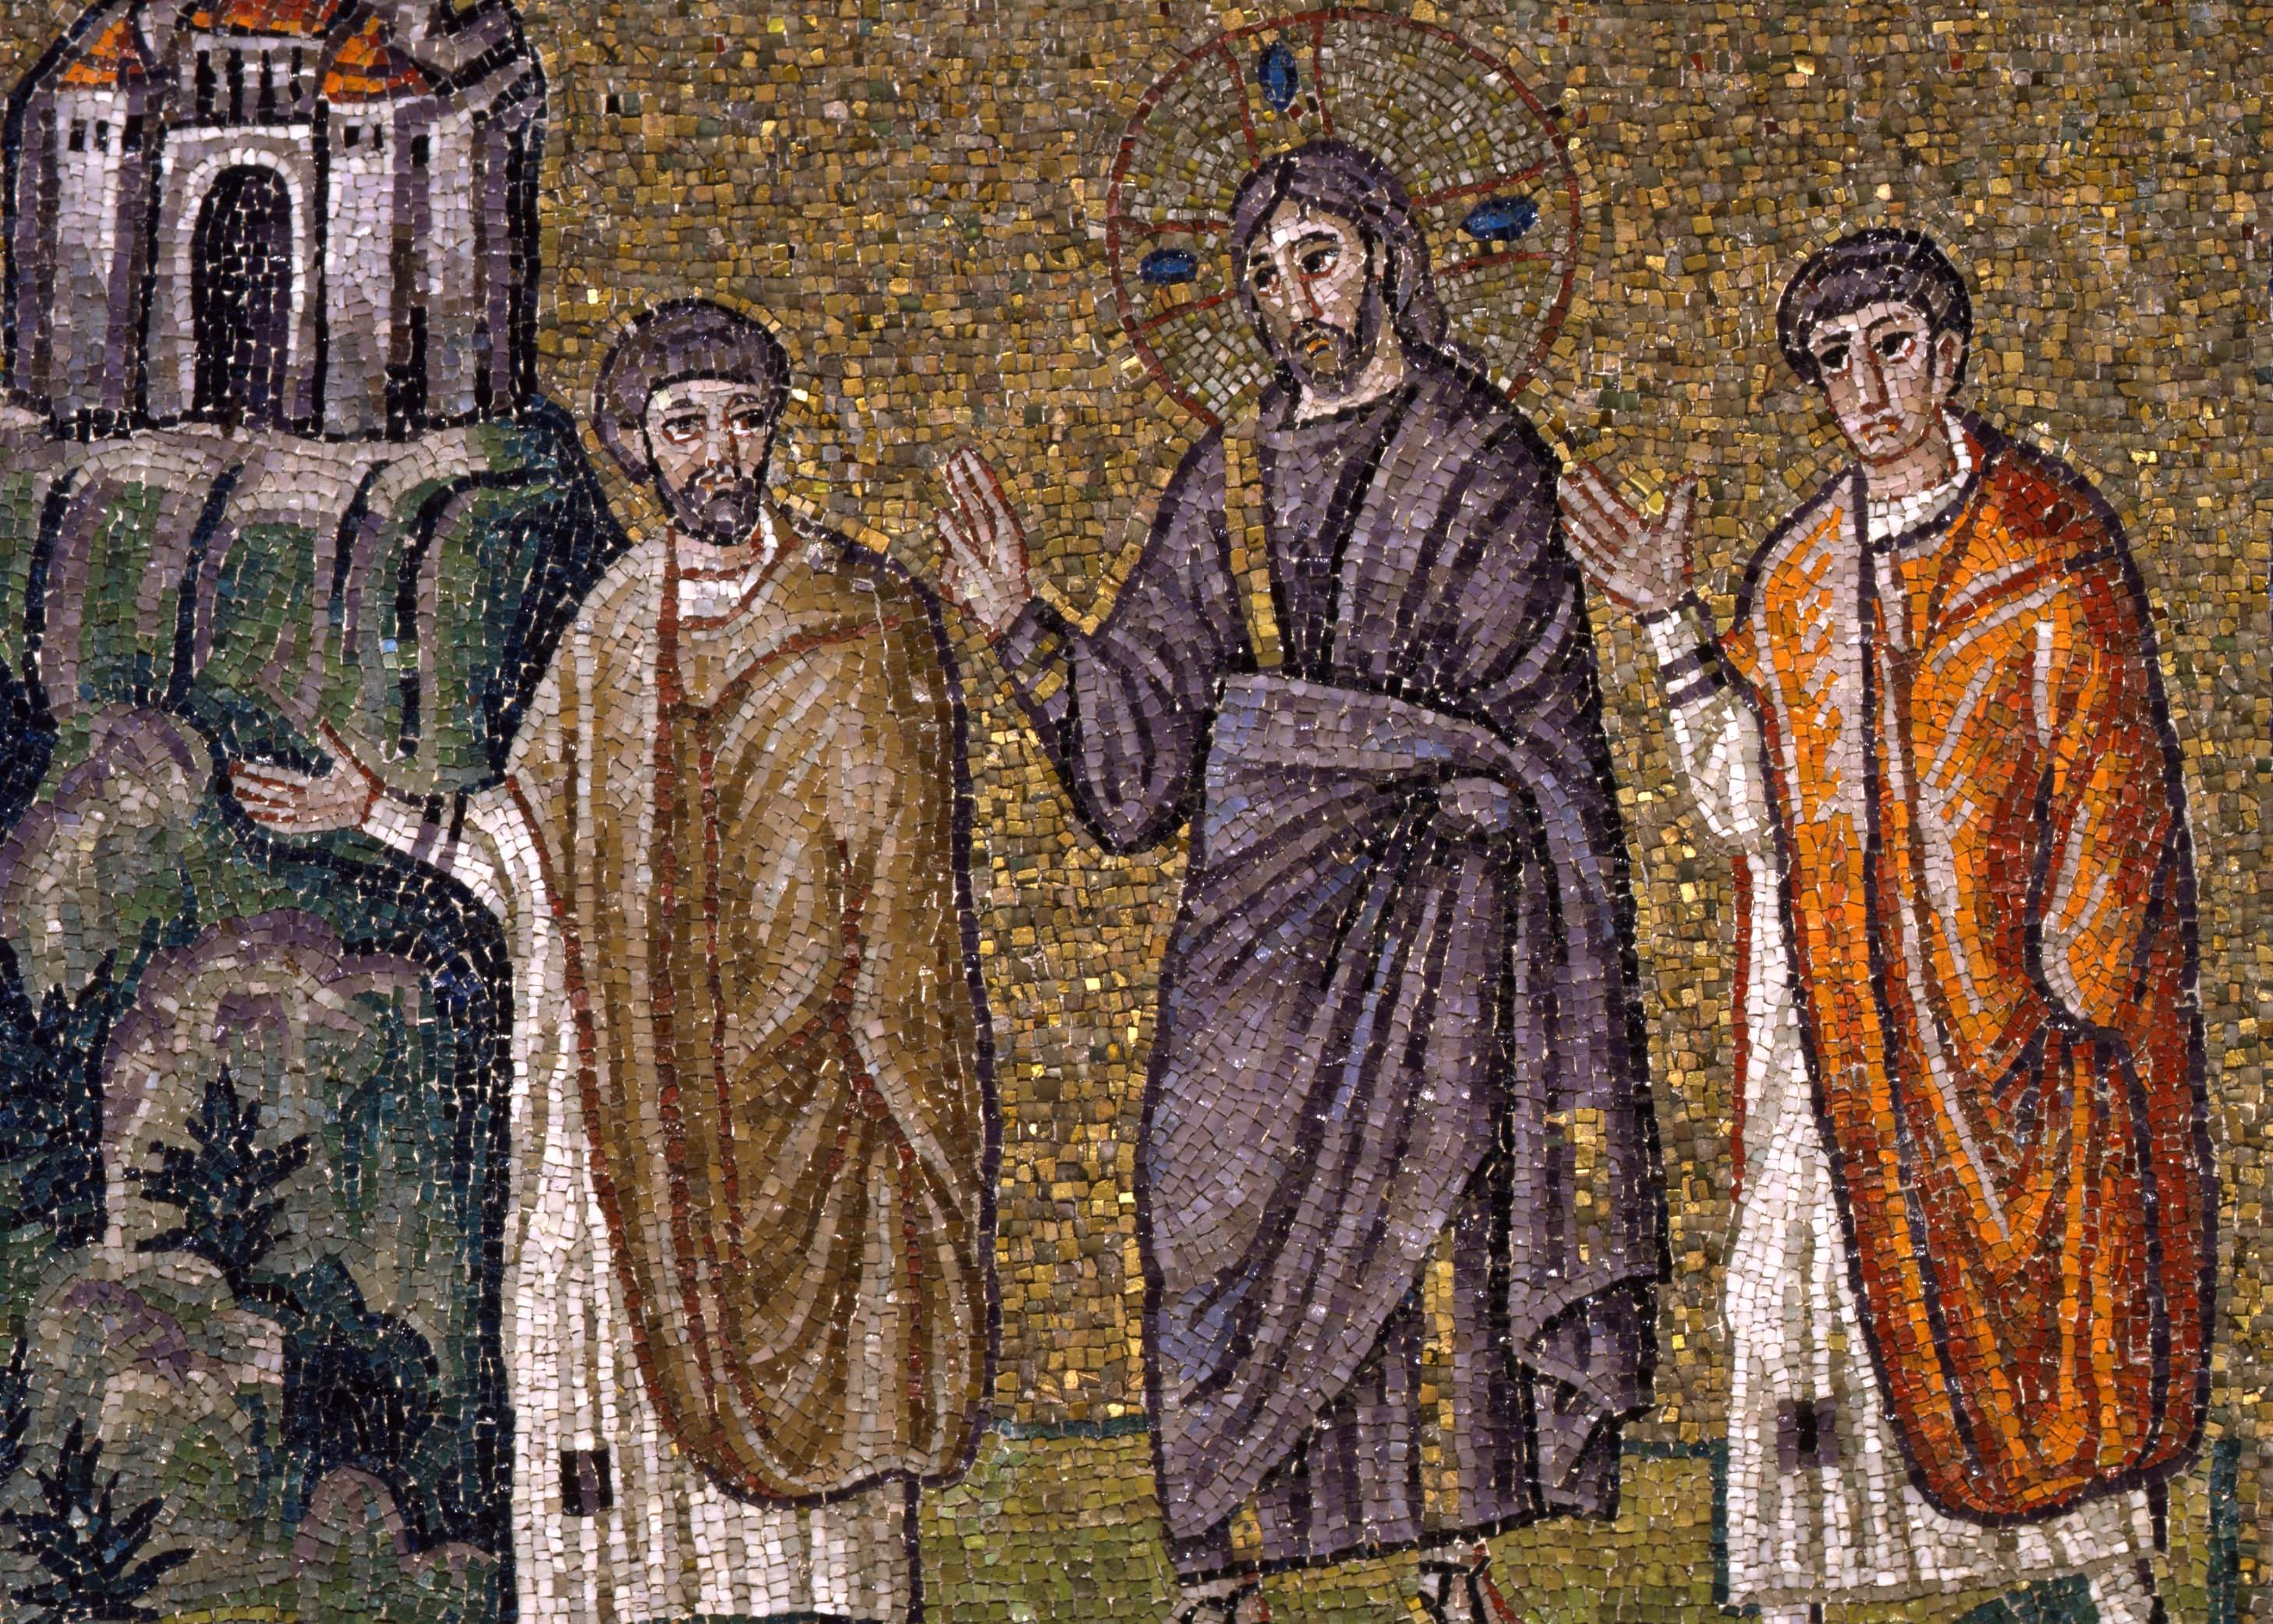
\includegraphics[width=8cm]{emmaus.jpg}
%\end{center}

\vfill

\begin{center}
%Ad usum et secundum consuetudines chori \guillemotright{}Conventus Choralis\guillemotleft.

%Editio Sancti Wolfgangi \annusEditionis
\end{center}

\pagebreak

\renewcommand{\headrulewidth}{0pt} % no horiz. rule at the header
\fancyhf{}
\pagestyle{fancy}

\pars{Oratio ante divinum Officium.}

\lettrine{{\color{red}A}}{peri,} Dómine, os meum ad benedicéndum nomen sanctum tuum:
munda quoque cor meum ab ómnibus vanis, pervérsis, et aliénis
cogitatiónibus:
intelléctum illúmina, afféctum inflámma,
ut digne, atténte ac devóte hoc Offícium recitáre váleam,
et exaudíri mérear ante conspéctum Divínæ Maiestátis tuæ.
Per Christum, Dóminum nostrum.
\Rbardot{} Amen.

Dómine, in unióne illíus divínæ intentiónis,
qua ipse in terris laudes Deo persolvísti,
has tibi Horas \rubricatum{(vel \textnormal{hanc tibi Horam})} persólvo.

%\trOratioAnteOfficium

\vfill

\pars{Oratio post divinum Officium.}

\rubrica{
  Orationem sequentem devote post Officium recitantibus
  Leo Papa X. defectus, et culpas in eo persolvendo ex humana
  fragilitate contractas, indulsit, et dicitur flexis genibus.
}

\lettrine{{\color{red}S}}{acrosánctæ} et indivíduæ Trinitáti,
crucifíxi Dómini nostri Iesu Christi humanitáti,
beatíssimæ et gloriosíssimæ sempérque Vírginis Maríæ
fecúndæ integritáti, 
et ómnium Sanctórum universitáti
sit sempitérna laus, honor, virtus et glória
ab omni creatúra,
nobísque remíssio ómnium peccatórum,
per infiníta sǽcula sæculórum.
\Rbardot{} Amen.

\noindent \Vbardot{} Beáta víscera Maríæ Virginis, quæ portavérunt
ætérni Patris Fílium.\\
\Rbardot{} Et beáta úbera, quæ lactavérunt Christum Dominum.

\rubrica{Et dicitur secreto \textnormal{Pater noster.} et \textnormal{Ave María.}}

%\trOratioPostOfficium

\vfill

\hora{Ad I. Vesperas.} %%%%%%%%%%%%%%%%%%%%%%%%%%%%%%%%%%%%%%%%%%%%%%%%%%%%%
%\sideThumbs{I. Vesperæ}

\cantusSineNeumas

\vspace{0.5cm}
\grechangedim{interwordspacetext}{0.18 cm plus 0.15 cm minus 0.05 cm}{scalable}%
\cuminitiali{}{temporalia/deusinadiutorium-solemnis.gtex}
\grechangedim{interwordspacetext}{0.22 cm plus 0.15 cm minus 0.05 cm}{scalable}%

\vfill
\pagebreak

\pars{Psalmus 1.} \scriptura{Ps. 144, 13; \textbf{H100}}

\vspace{-4mm}

\antiphona{VII c\textsuperscript{2}}{temporalia/ant-regnumtuum.gtex}

\scriptura{Psalmus 144, 10-21.}

\initiumpsalmi{temporalia/ps144ii-initium-vii-c2-auto.gtex}

%\psalmusEtTranslatioT{temporalia/ps144ii-VII-comb.tex}{10cm}
\input{temporalia/ps144ii-VII.tex} \Abardot{}

\vspace{-1cm}

\vfill
\pagebreak

\pars{Psalmus 2.} \scriptura{Ps. 145, 2; \textbf{H100}}

\vspace{-4mm}

\antiphona{IV E}{temporalia/ant-laudabodeum.gtex}

\scriptura{Psalmus 145.}

\initiumpsalmi{temporalia/ps145-initium-iv-E-auto.gtex}

%\psalmusEtTranslatioT{temporalia/ps145-VII-comb.tex}{10cm}
\input{temporalia/ps145-VII.tex} \Abardot{}

\vfill
\pagebreak

\pars{Psalmus 3.} \scriptura{Ps. 146, 1; \textbf{H101}}

\vspace{-4mm}

\antiphona{VIII a}{temporalia/ant-deonostro.gtex}

\scriptura{Psalmus 146.}

\initiumpsalmi{temporalia/ps146-initium-viii-A-auto.gtex}

%\psalmusEtTranslatioT{temporalia/ps146-VII-comb.tex}{10cm}
\input{temporalia/ps146-VII.tex} \Abardot{}

\vfill
\pagebreak

\pars{Psalmus 4.} \scriptura{Ps. 147, 1}

\vspace{-4mm}

\antiphona{E}{temporalia/ant-laudajerusalem.gtex}

\scriptura{Psalmus 147.}

\initiumpsalmi{temporalia/ps147-initium-e-auto.gtex}

%\psalmusEtTranslatioT{temporalia/ps147-VII-comb.tex}{10cm}
\input{temporalia/ps147-VII.tex} \Abardot{}

\vfill
\pagebreak

\pars{Capitulum.} \scriptura{Rom. 11, 33}

\grechangedim{interwordspacetext}{0.12 cm plus 0.15 cm minus 0.05 cm}{scalable}%
\cuminitiali{}{temporalia/capitulum-OAltitudo.gtex}
\grechangedim{interwordspacetext}{0.22 cm plus 0.15 cm minus 0.05 cm}{scalable}

% preklad Jeruz. bible
%\trCapituliI

\vfill

\pars{Responsorium breve.} \scriptura{Ps. 146, 5}

\cuminitiali{VI}{temporalia/resp-magnusdominusnoster.gtex}

%\trResp

\vfill
\pagebreak

\pars{Hymnus} \scriptura{Ambrosius (\olddag{} 397)}

\cuminitiali{I}{temporalia/hym-OLuxBeata-aestivalis.gtex}
\vspace{-3mm}
%\input{hym-OLuxBeata-bohtext.tex}

\vfill
%\pagebreak

\pars{Versus.}

% Versus. %%%
\sineinitiali{temporalia/versus-vespertina.gtex}

%\noindent \trVersus

\vfill
\pagebreak

\magnificati

\vfill
\pagebreak

%\sideThumbs{{\scriptsize{}Fine horarum}}

\anteOrationem

\pagebreak

% Oratio. %%%
\oratioLaudes

\vspace{-1mm}
%\trOrationisI

\vfill

\rubrica{Hebdomadarius dicit iterum Dominus vobiscum, vel cantor dicit:}

\vspace{2mm}

\sineinitiali{temporalia/domineexaudi.gtex}

\rubrica{Postea cantatur a cantore:}

\vspace{2mm}

\cuminitiali{I}{temporalia/benedicamus-dominica-perannum.gtex}

\vspace{1mm}

\vfill
\pagebreak

\hora{Ad Matutinum.} %%%%%%%%%%%%%%%%%%%%%%%%%%%%%%%%%%%%%%%%%%%%%%%%%%%%%
%\sideThumbs{Matutinum}

\vspace{2mm}

\cuminitiali{}{temporalia/dominelabiamea.gtex}

\vspace{2mm}

\pars{Invitatorium.} \scriptura{Ps. 94, 1; Psalmus 94}

\vspace{-6mm}

\antiphona{E}{temporalia/inv-veniteexsultemus.gtex}

\vfill
\pagebreak

\pars{Hymnus.} \scriptura{Adamus Sancti Victoris (\olddag 1146)}

\vspace{-5mm}

\antiphona{VII}{temporalia/hym-SalveDies.gtex}

\scriptura{Non dicitur \textnormal{Amen} in fine.}
%{
%\vspace{-5mm}
%\setlength{\columnsep}{0pt} % prostor mezi sloupci
%\input{hym-SalveDies-bohtext.tex}
%\setlength{\columnsep}{30pt} % prostor mezi sloupci
%}

\vfill
\pagebreak

\iffalse
\subhora{In I. Nocturno}

\pars{Psalmus 1.} \scriptura{\textbf{H230}}

%\vspace{-5mm}

\antiphona{V a}{temporalia/ant-alleluialapis.gtex}

%\vspace{-5mm}

\scriptura{Ps. 1}

%\vspace{-2mm}

\initiumpsalmi{temporalia/ps1-initium-v-a-auto.gtex}

%\psalmusEtTranslatioT{temporalia/ps1-comb.tex}{10cm}

\input{temporalia/ps1.tex}

\vfill
\pagebreak

\pars{Psalmus 2.}

\scriptura{Ps. 2}

\initiumpsalmi{temporalia/ps2-initium-v-a-auto.gtex}

%\psalmusEtTranslatioT{temporalia/ps2-comb.tex}{10cm}

\input{temporalia/ps2.tex}

\vfill
\pagebreak

\pars{Psalmus 3.}

\scriptura{Ps. 3}

\initiumpsalmi{temporalia/ps3-initium-v-a-auto.gtex}

%\psalmusEtTranslatioT{temporalia/ps3-comb.tex}{10cm}

\input{temporalia/ps3.tex}

\vfill

\antiphona{}{temporalia/ant-alleluialapis.gtex}

\vfill
\pagebreak
\fi

\noindent \Vbardot{} Memor fui nocte nóminis tui, Dómine.
\noindent \Rbardot{} Et custodívi legem tuam.

\vspace{5mm}

\sineinitiali{temporalia/oratiodominica-mat.gtex}

\vspace{5mm}

\pars{Absolutio.}

\cuminitiali{}{temporalia/absolutio-exaudi.gtex}

\vfill
\pagebreak

\cuminitiali{}{temporalia/benedictio-solemn-benedictione.gtex}

\vspace{7mm}

\lectioi

\noindent \Vbardot{} Tu autem, Dómine, miserére nobis.
\noindent \Rbardot{} Deo grátias.

\vfill
\pagebreak

\responsoriumi

\vfill
\pagebreak

\cuminitiali{}{temporalia/benedictio-solemn-unigenitus.gtex}

\vspace{7mm}

\lectioii

\noindent \Vbardot{} Tu autem, Dómine, miserére nobis.
\noindent \Rbardot{} Deo grátias.

\vfill
\pagebreak

\responsoriumii

\vfill
\pagebreak

\cuminitiali{}{temporalia/benedictio-solemn-spiritus.gtex}

\vspace{7mm}

\lectioiii

\noindent \Vbardot{} Tu autem, Dómine, miserére nobis.
\noindent \Rbardot{} Deo grátias.

\vfill
\pagebreak

\responsoriumiii

\vfill
\pagebreak

\iffalse
\subhora{In II. Nocturno}

\pars{Psalmus 4.} \scriptura{Io. 20, 15; \textbf{H241}}

%\vspace{-5mm}

\antiphona{V a}{temporalia/ant-alleluiaquem.gtex}

%\vspace{-5mm}

\scriptura{Ps. 8}

%A\vspace{-2mm}

\initiumpsalmi{temporalia/ps8-initium-v-a-auto.gtex}

%\psalmusEtTranslatioT{temporalia/ps8-comb.tex}{10cm}

\input{temporalia/ps8.tex}

\vfill
\pagebreak

\pars{Psalmus 5.}

\scriptura{Ps. 9, 2-11}

\initiumpsalmi{temporalia/ps9ii_xi-initium-v-a-auto.gtex}

%\psalmusEtTranslatioT{temporalia/ps9ii_xi-comb.tex}{10cm}

\input{temporalia/ps9ii_xi.tex}

\vfill
\pagebreak

\pars{Psalmus 6.}

\scriptura{Ps. 9, 12-21}

\initiumpsalmi{temporalia/ps9xii_xxi-initium-v-a-auto.gtex}

%\psalmusEtTranslatioT{temporalia/ps9xii_xxi-comb.tex}{10cm}

\input{temporalia/ps9xii_xxi.tex}

\vfill

\antiphona{}{temporalia/ant-alleluiaquem.gtex}

\vfill
\pagebreak
\fi

\noindent \Vbardot{} Média nocte surgébam ad confiténdum tibi.
\noindent \Rbardot{} Super iudícia iustificatiónis tuæ.

\vspace{5mm}

\sineinitiali{temporalia/oratiodominica-mat.gtex}

\vspace{5mm}

\pars{Absolutio.}

\cuminitiali{}{temporalia/absolutio-ipsius.gtex}

\vfill
\pagebreak

\cuminitiali{}{temporalia/benedictio-solemn-deus.gtex}

\vspace{7mm}

\lectioiv

\noindent \Vbardot{} Tu autem, Dómine, miserére nobis.
\noindent \Rbardot{} Deo grátias.

\vfill
\pagebreak

\responsoriumiv

\vfill
\pagebreak

\cuminitiali{}{temporalia/benedictio-solemn-christus.gtex}

\vspace{7mm}

\lectiov

\noindent \Vbardot{} Tu autem, Dómine, miserére nobis.
\noindent \Rbardot{} Deo grátias.

\vfill
\pagebreak

\responsoriumv

\vfill
\pagebreak

\cuminitiali{}{temporalia/benedictio-solemn-ignem.gtex}

\vspace{7mm}

\lectiovi

\noindent \Vbardot{} Tu autem, Dómine, miserére nobis.
\noindent \Rbardot{} Deo grátias.

\vfill
\pagebreak

\responsoriumvi

\vfill
\pagebreak

\iffalse
\subhora{In III. Nocturno}

\pars{Psalmus 7.} \scriptura{Cf. Io. 20, 15; \textbf{H241}}

\vspace{-5mm}

\antiphona{V a}{temporalia/ant-alleluianoli.gtex}

\vspace{-4mm}

\scriptura{Ps. 9, 22-32}

%\vspace{-2mm}

\initiumpsalmi{temporalia/ps9xxii_xxxii-initium-v-a-auto.gtex}

%\psalmusEtTranslatioT{temporalia/ps9xxii_xxxii-comb.tex}{10cm}

\input{temporalia/ps9xxii_xxxii.tex}

\vfill
\pagebreak

\pars{Psalmus 8.}

\scriptura{Ps. 9, 33-39}

\initiumpsalmi{temporalia/ps9xxxiii_xxxix-initium-v-a-auto.gtex}

%\psalmusEtTranslatioT{temporalia/ps9xxxiii_xxxix-comb.tex}{10cm}

\input{temporalia/ps9xxxiii_xxxix.tex}

\vfill
\pagebreak

\pars{Psalmus 9.}

\scriptura{Ps. 10}

\initiumpsalmi{temporalia/ps10-initium-v-a-auto.gtex}

%\psalmusEtTranslatioT{temporalia/ps10-comb.tex}{10cm}

\input{temporalia/ps10.tex}

\vfill

\antiphona{}{temporalia/ant-alleluianoli.gtex}

\vfill
\pagebreak
\fi

\noindent \Vbardot{} Prævenérunt óculi mei ad te dilúculo.
\noindent \Rbardot{} Ut meditárer elóquia tua, Dómine.

\vspace{5mm}

\sineinitiali{temporalia/oratiodominica-mat.gtex}

\vspace{5mm}

\pars{Absolutio.}

\cuminitiali{}{temporalia/absolutio-avinculis.gtex}

\vfill
\pagebreak

\cuminitiali{}{temporalia/benedictio-solemn-evangelica.gtex}

\vspace{7mm}

\lectiovii

\noindent \Vbardot{} Tu autem, Dómine, miserére nobis.
\noindent \Rbardot{} Deo grátias.

\vfill
\pagebreak

\responsoriumvii

\vfill
\pagebreak

\cuminitiali{}{temporalia/benedictio-solemn-divinum.gtex}

\vspace{7mm}

\lectioviii

\noindent \Vbardot{} Tu autem, Dómine, miserére nobis.
\noindent \Rbardot{} Deo grátias.

\vfill
\pagebreak

\responsoriumviii

\vfill
\pagebreak

\cuminitiali{}{temporalia/benedictio-solemn-adsocietatem.gtex}

\vspace{7mm}

\lectioix

\noindent \Vbardot{} Tu autem, Dómine, miserére nobis.
\noindent \Rbardot{} Deo grátias.

\vfill
\pagebreak

% Te Deum

{
\pars{Hymnus Ambrosianus} \scriptura{Tonus Solemnis}

\vspace{-2mm}

\grechangedim{interwordspacetext}{0.26 cm plus 0.15 cm minus 0.05 cm}{scalable}%
\cuminitiali{III}{temporalia/tedeum-solemnis-gn.gtex}
\grechangedim{interwordspacetext}{0.22 cm plus 0.15 cm minus 0.05 cm}{scalable}%
}

\vfill
\pagebreak

\rubrica{Reliqua omittuntur, nisi Laudes separandæ sint.}

\pars{Oratio}

\noindent \Vbardot{} Dómine, exáudi oratiónem meam.

\noindent \Rbardot{} Et clamor meus ad te véniat.

Orémus:

\oratioLaudes

\vspace{7mm}

\pars{Conclusio}

\noindent \Vbardot{} Dómine, exáudi oratiónem meam.

\noindent \Rbardot{} Et clamor meus ad te véniat.

\noindent \Vbardot{} Benedicámus Dómino, allelúia, allelúia.

\noindent \Rbardot{} Deo grátias, allelúia, allelúia.

\noindent \Vbardot{} Fidélium ánimæ per misericórdiam Dei requiéscant in pace.

\noindent \Rbardot{} Amen.

\vfill
\pagebreak

\hora{Ad Laudes.} %%%%%%%%%%%%%%%%%%%%%%%%%%%%%%%%%%%%%%%%%%%%%%%%%%%%%
%\sideThumbs{Laudes}

\cantusSineNeumas

\vspace{0.5cm}
\grechangedim{interwordspacetext}{0.18 cm plus 0.15 cm minus 0.05 cm}{scalable}%
\cuminitiali{}{temporalia/deusinadiutorium-alter.gtex}
\grechangedim{interwordspacetext}{0.22 cm plus 0.15 cm minus 0.05 cm}{scalable}%

\vfill
%\pagebreak

\pars{Psalmus 1.}

\vspace{-4mm}

\antiphona{VI F}{temporalia/ant-alleluia1.gtex}

\scriptura{Psalmus 50.}

\initiumpsalmi{temporalia/ps50-initium-vi-F-auto.gtex}

%\psalmusEtTranslatioT{temporalia/ps50-I-comb.tex}{10cm}
\input{temporalia/ps50-I.tex}

\vfill
\pagebreak

\pars{Psalmus 2.}

\scriptura{Psalmus 117.}

\initiumpsalmi{temporalia/ps117-initium-vi-F-auto.gtex}

%\psalmusEtTranslatioT{temporalia/ps117-I-comb.tex}{10cm}
\input{temporalia/ps117-I.tex}

\vfill
\pagebreak

\pars{Psalmus 3.}

\scriptura{Psalmus 62.}

\initiumpsalmi{temporalia/ps62-initium-vi-F-auto.gtex}

%\psalmusEtTranslatioT{temporalia/ps62-I-comb.tex}{10cm}
\input{temporalia/ps62-I.tex}

\vfill

\vspace{-6mm}

\antiphona{}{temporalia/ant-alleluia1.gtex} % repeat the antiphon - new page

\vfill
\pagebreak

\pars{Psalmus 4.} \scriptura{Dan. 3, 22-26; \textbf{H422}}

\vspace{-4mm}

\antiphona{VIII G}{temporalia/ant-trespueri.gtex}

\scriptura{Canticum trium puerorum, Dan. 3, 57-88 et 56}

\initiumpsalmi{temporalia/dan3-initium-viii-G-auto.gtex}

%\psalmusEtTranslatioT{temporalia/dan3-comb.tex}{10cm}
\input{temporalia/dan3.tex}

\rubrica{Hic non dicitur Gloria Patri, neque Amen.}

\vfill

\vspace{-6mm}

\antiphona{}{temporalia/ant-trespueri.gtex} % repeat the antiphon - new page

\vfill
\pagebreak

\pars{Psalmus 5.}

\vspace{-4mm}

\antiphona{VIII G}{temporalia/ant-alleluia2.gtex}

\scriptura{Psalmus 148.}

\initiumpsalmi{temporalia/ps148-initium-viii-G-auto.gtex}

%\psalmusEtTranslatioT{temporalia/ps148-I-comb.tex}{10cm}
\input{temporalia/ps148-I.tex}

\rubrica{Hic non dicitur Gloria Patri.}

\vfill
\pagebreak

%
\scriptura{Psalmus 149.}

\initiumpsalmi{temporalia/ps149-initium-viii-G-auto.gtex}

%\psalmusEtTranslatioT{temporalia/ps149-I-comb.tex}{10cm}
\input{temporalia/ps149-I.tex}

\rubrica{Hic non dicitur Gloria Patri.}

\vfill
\pagebreak

%
\scriptura{Psalmus 150.}

\initiumpsalmi{temporalia/ps150-initium-viii-G-auto.gtex}

%\psalmusEtTranslatioT{temporalia/ps150-I-comb.tex}{10cm}
\input{temporalia/ps150-I.tex}

\vfill

\vspace{-6mm}

\antiphona{}{temporalia/ant-alleluia2.gtex} % repeat the antiphon - new page

\vfill
\pagebreak

\pars{Capitulum.} \scriptura{Ac. 7, 12}

\grechangedim{interwordspacetext}{0.12 cm plus 0.15 cm minus 0.05 cm}{scalable}%
\cuminitiali{}{temporalia/capitulum-Benedictio.gtex}
\grechangedim{interwordspacetext}{0.22 cm plus 0.15 cm minus 0.05 cm}{scalable}

% preklad Jeruz. bible
%\trCapituliI

\vfill

\pars{Responsorium breve.} \scriptura{Ps. 118, 36-37}

\cuminitiali{IV}{temporalia/resp-inclinacormeum.gtex}

%\trResp

\vfill
\pagebreak

\pars{Hymnus} \scriptura{Gregorius Magnus (\olddag{} 604)}

\cuminitiali{IV}{temporalia/hym-EcceJamNoctis.gtex}
\vspace{-3mm}
%\input{hym-EcceJamNocis-bohtext.tex}

\vfill
%\pagebreak

\pars{Versus.} \scriptura{Ps. 92, 1}

% Versus. %%%
\sineinitiali{temporalia/versus-dominusregnavit.gtex}

%\noindent \trVersus

\vfill
\pagebreak

\benedictus

\vspace{-1cm}

\vfill
\pagebreak

%\sideThumbs{{\scriptsize{}Fine horarum}}

\anteOrationem

\pagebreak

% Oratio. %%%
\oratioLaudes

\vspace{-1mm}
%\trOrationisI

\vfill

\rubrica{Hebdomadarius dicit iterum Dominus vobiscum, vel cantor dicit:}

\vspace{2mm}

\sineinitiali{temporalia/domineexaudi.gtex}

\rubrica{Postea cantatur a cantore:}

\vspace{2mm}

\cuminitiali{I}{temporalia/benedicamus-dominica-perannum.gtex}

\vspace{1mm}

\vfill
\pagebreak

\hora{Ad II. Vesperas.} %%%%%%%%%%%%%%%%%%%%%%%%%%%%%%%%%%%%%%%%%%%%%%%%%%%%%
%\sideThumbs{II. Vesperæ}

\cantusSineNeumas

%\vspace{0.5cm}
\grechangedim{interwordspacetext}{0.18 cm plus 0.15 cm minus 0.05 cm}{scalable}%
\cuminitiali{}{temporalia/deusinadiutorium-solemnis.gtex}
\grechangedim{interwordspacetext}{0.22 cm plus 0.15 cm minus 0.05 cm}{scalable}%

\vfill
%\pagebreak

\vspace{-2mm}

\pars{Psalmus 1.} \scriptura{Ps. 109, 1; \textbf{H91}}

\vspace{-4mm}

\antiphona{VII c\textsuperscript{2}}{temporalia/ant-dixitdominus.gtex}

\vspace{-4mm}

\scriptura{Psalmus 109.}

\initiumpsalmi{temporalia/ps109-initium-vii-c2-auto.gtex}

%\psalmusEtTranslatioT{temporalia/ps109-I-comb.tex}{10cm}
\input{temporalia/ps109-I.tex} \Abardot{}

\vspace{-1cm}

\vfill
\pagebreak

\pars{Psalmus 2.} \scriptura{Ps. 110, 8; \textbf{H91}}

\vspace{-4mm}

\antiphona{IV g}{temporalia/ant-fideliaomnia.gtex}

\scriptura{Psalmus 110.}

\initiumpsalmi{temporalia/ps110-initium-iv-g-auto.gtex}

%\psalmusEtTranslatioT{temporalia/ps110-I-comb.tex}{10cm}
\input{temporalia/ps110-I.tex} \Abardot{}

\vfill
\pagebreak

\pars{Psalmus 3.} \scriptura{Ps. 111, 1; \textbf{H92}}

\vspace{-4mm}

\antiphona{IV a}{temporalia/ant-inmandatis.gtex}

\scriptura{Psalmus 111.}

\initiumpsalmi{temporalia/ps111-initium-iv-a-auto.gtex}

%\psalmusEtTranslatioT{temporalia/ps111-I-comb.tex}{10cm}
\input{temporalia/ps111-I.tex} \Abardot{}

\vfill
\pagebreak

\pars{Psalmus 4.} \scriptura{Ps. 112, 2; \textbf{H92}}

\vspace{-4mm}

\antiphona{VII c}{temporalia/ant-sitnomendomini.gtex}

\scriptura{Psalmus 112.}

\initiumpsalmi{temporalia/ps112-initium-vii-c-auto.gtex}

%\psalmusEtTranslatioT{temporalia/ps112-I-comb.tex}{10cm}
\input{temporalia/ps112-I.tex} \Abardot{}

\vfill
\pagebreak

\pars{Capitulum.} \scriptura{2 Cor. 1, 3-4}

\grechangedim{interwordspacetext}{0.12 cm plus 0.15 cm minus 0.05 cm}{scalable}%
\cuminitiali{}{temporalia/capitulum-BenedictusDeus.gtex}
\grechangedim{interwordspacetext}{0.22 cm plus 0.15 cm minus 0.05 cm}{scalable}

% preklad Jeruz. bible
%\trCapituliI

\vfill

\pars{Responsorium breve.} \scriptura{Ps. 103, 24}

\cuminitiali{VI}{temporalia/resp-quammagnificata.gtex}

%\trResp

\vfill
\pagebreak

\pars{Hymnus} \scriptura{Gregorius Magnus (\olddag{} 604)}

\cuminitiali{I}{temporalia/hym-LucisCreator-aestivalis.gtex}
\vspace{-3mm}
%\begin{translatioMulticol}{3}
Tvůrce světa předobrý,\\
tys ustanovil denní řád\\
a proudy světla rozhodil,\\
když světu základy jsi klad.\\
\\
A spojils ráno s večerem\\
a dnem tu dobu nazýváš;\\
hle padá temné noci stín -\\
slyš prosbu, vyslyš nářek náš.\columnbreak

Ach, nedej, by nás stihla smrt,\\
když svědomí nám tíží hřích,\\
když nemyslíme na věčnost\\
v té síti hříchů šalebných.\\
\\
Vzbuď naši touhu po nebi,\\
kde věčný život čeká nás,\\
a pomoz odložit vše zlé\\
a smýti z duše každý kaz.\columnbreak

To splň nám, dobrý Otče náš,\\
i ty, jenž rovné božství máš,\\
i Duchu, který těšíš nás\\
a vládneš, Bože, v každý čas.\\
Amen. 
\end{translatioMulticol}


\vfill
%\pagebreak

\pars{Versus.} \scriptura{Ps. 140, 2}

% Versus. %%%
\sineinitiali{temporalia/versus-dirigatur.gtex}

%\noindent \trVersus

\vfill
\pagebreak

\magnificatii

\vfill
\pagebreak

%\sideThumbs{{\scriptsize{}Fine horarum}}

\anteOrationem

\pagebreak

% Oratio. %%%
\oratioLaudes

\vspace{-1mm}
%\trOrationisI

\vfill

\rubrica{Hebdomadarius dicit iterum Dominus vobiscum, vel cantor dicit:}

\vspace{2mm}

\sineinitiali{temporalia/domineexaudi.gtex}

\rubrica{Postea cantatur a cantore:}

\vspace{2mm}

\cuminitiali{I}{temporalia/benedicamus-dominica-perannum.gtex}

\vspace{1mm}

\end{document}

